% asset_id: AS2ModellingInMechanicsTIKZ-004
\documentclass[tikz,border=8pt]{standalone}
\usepackage{amsmath}
\usetikzlibrary{arrows.meta}
\begin{document}
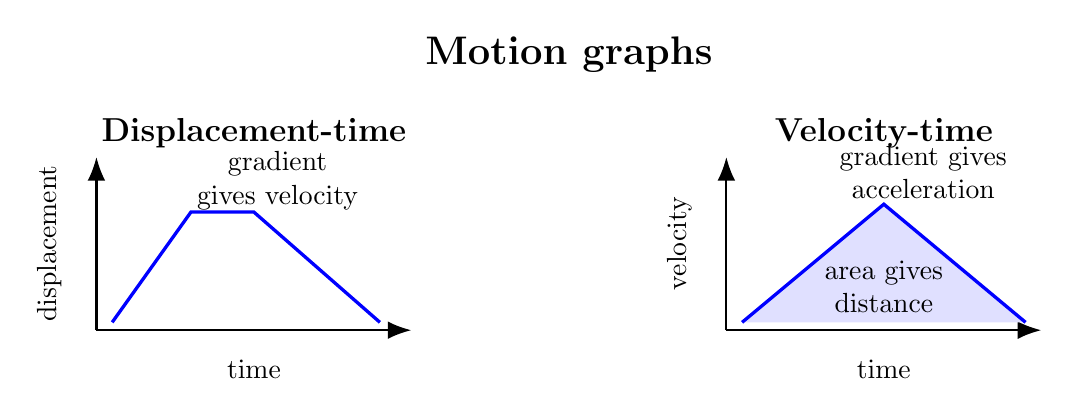
\begin{tikzpicture}[axis/.style={-{Latex[length=3mm]}, thick}, graph/.style={very thick, blue}]
\node[font=\Large\bfseries] at (0,3.5) {Motion graphs};
\node[font=\large\bfseries] at (-4,2.5) {Displacement-time};\draw[axis] (-6,0) -- (-2,0);\draw[axis] (-6,0) -- (-6,2.2);\node at (-4,-0.5) {time};\node[rotate=90] at (-6.6,1.1) {displacement};\draw[graph] (-5.8,0.1) -- (-4.8,1.5) -- (-4.0,1.5) -- (-2.4,0.1);\node[align=center] at (-3.7,1.9) {gradient\\gives velocity};
\node[font=\large\bfseries] at (4,2.5) {Velocity-time};\draw[axis] (2,0) -- (6,0);\draw[axis] (2,0) -- (2,2.2);\node at (4,-0.5) {time};\node[rotate=90] at (1.4,1.1) {velocity};\fill[blue!12] (2.2,0.1) -- (4,1.6) -- (5.8,0.1) -- cycle;\draw[graph] (2.2,0.1) -- (4,1.6) -- (5.8,0.1);\node[align=center] at (4.5,2.0) {gradient gives\\acceleration};\node[align=center] at (4,0.55) {area gives\\distance};
\end{tikzpicture}
\end{document}
